\section{Simulation of Data}\label{sec:dataset}
To test the performance of the algorithms simulated data, corresponding to the model $\textbf{Y}=\textbf{A}\textbf{X}$, is needed. All data sets are simulated based on the following approach, satisfying the sufficient conditions for recovery, displayed in theorem \ref{th:conditions}. 
A source matrix $\textbf{X}\in \mathbb{R}^{N\times L}$ is constructed, such that each row makes an independent signal which varies over $L$ times samples or a zero row. As such the non zero rows of $\textbf{X}$ are mutually orthogonal, which fulfils the first conditions of theorem \ref{th:conditions}.   
Then a mixing matrix $\textbf{A}\in \mathbb{R}^{M\times N}$ is constructed with equally distributed and independent entries. As such the source signals are randomly mixed and the mixing matrix fulfils the second condition of theorem \ref{th:conditions}.
With known $\textbf{A}$ and $\textbf{X}$ the a dataset $\textbf{Y}\in \mathbb{R}^{M\times L}$ is simulated according to the model, by the matrix product $\textbf{Y}= \textbf{AX}$.  

Two different data sets are simulated.
One simple data set with simple and predictable source signals to ensure a solution and easy visualisation.
Another data set with randomised and fluctuating source signals to resemble realistic EEG measurements.

\subsection{Simple Data Set}
The simple data set is specified by $N = 5$, $k=4$, $M = 3$ and $L = 100$. That is a source matrix $\textbf{X}$ with $4$ independent signals and $1$ zero row which is mixed into a data set with $3$ measurement per sample.       
The 5 rows of $\textbf{X}$ are defined by 
\begin{itemize}
\item[1.] a sinus signal $\sin(2t)$
\item[2.] zero row
\item[3.] a sawtooth signal with period $2 \pi t$
\item[4.] a sinus signal $\sin(4t)$
\item[5.] a sign function of a sinus signal $\sin(3t)$
\end{itemize}
with $t$ being a time index defined in the interval $[0,4]$ with $L$ samples. Each of the four signal are randomly drawn and used to construct a source matrix $\mathbf{X}$ of size $k \times L$.
The mixing matrix $\mathbf{A}$ of size $M \times k$ is randomly generated from a Gaussian distribution. 
By multiplying the source matrix and the mixing matrix the measurement matrix $\mathbf{Y}$ is achieved.
The simple data set then consist of $\{ \mathbf{Y}, \mathbf{X}, \mathbf{A} \}$.
In figure \ref{fig:mix} the source signals are plotted over the measurement signal $\mathbf{Y}$ to illustrates how the sources signal are transformed by the mixing matrix $\textbf{A}$.
\begin{figure}[H]
\centering
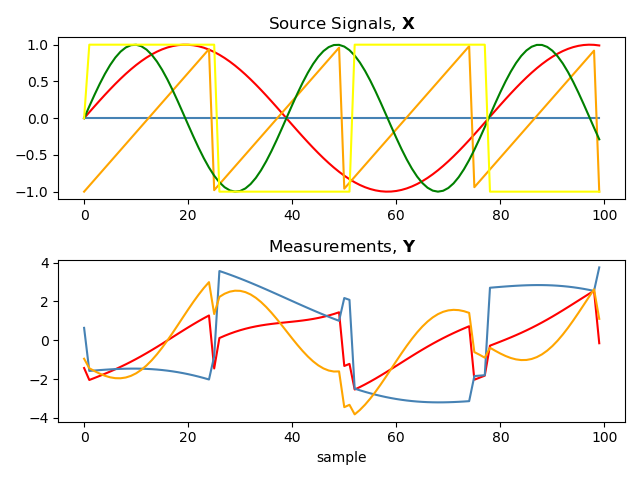
\includegraphics[scale=0.5]{figures/ch_6/simple_data.png}
\caption{This is a visualization of the measurement matrix $\mathbf{Y}$ from the simple data set for $M = 3$, $k=4$ and $L=1000$. As $k = 4$ there are four signals representing the measurement matrix $\mathbf{Y}$.}
\label{fig:mix}
\end{figure}
\noindent

\subsubsection{Autoregressive Data Set}
The second data set illustrate a more realistic data set.
The data set is constructed from four different autoregressive processes representing the sources of the source matrix $\mathbf{X}$ \todo{Skal lige finde en god måde at skrive dem ind på}: 
\begin{itemize}
\item[-] $\mathbf{x}^{t} = \mathbf{a1}^{t-1} \cdot \mathbf{x}^{t-1} + \mathbf{a1}^{t-2} \cdot \mathbf{x}^{t-2} + \mathbf{w1}_t$
\item[-] $\mathbf{x}^{t+1} = \mathbf{a2}_t \cdot \mathbf{x}_{t-1} + \mathbf{a}_t \cdot \mathbf{x}_t + \mathbf{w}_t$
\item[-] $\mathbf{x}_{t+1} = \mathbf{a}_t \cdot \mathbf{x}_{t-2} + \mathbf{a}_t \cdot \mathbf{x}_t + + \mathbf{a}_t \cdot \mathbf{x}_{t-1} \mathbf{w}_t$
\item[-] $\mathbf{x}_{t+1} = \mathbf{a}_t \cdot \mathbf{x}_t + \mathbf{a}_t \cdot \mathbf{x}_{t-3} + \mathbf{w}_t$
\end{itemize}
Each of the four autoregressive processes are randomly drawn and used to construct a source matrix $\mathbf{X}$ of size $k \times L$. 
The mixing matrix $\mathbf{A}$ of size $M \times k$ is randomly generated as the same way as the mixing matrix from the simple data set, from a Gaussian distribution. 
By multiplying the source matrix and the mixing matrix the measurement matrix $\mathbf{Y}$ is achieved.
The autoregressive data set then consist of $\{ \mathbf{Y}, \mathbf{X}, \mathbf{A} \}$ which are the true values of the MMV model.

An illustration of the autoregressive data set can be seen in figure \ref{fig:AR}. The data set is constructed for $M = 3$, $k = 4$ and $L = 1000$.
\begin{figure}[H]
\centering
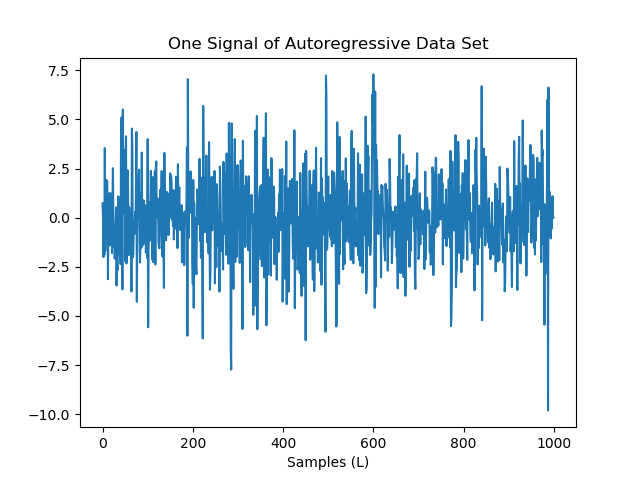
\includegraphics[scale=0.5]{figures/chapter6/AR_Data_m3_n4_k4_L1000.png}
\caption{This is a visualization of the first row of the measurement matrix $\mathbf{Y}$ from the autoregressive data set for $M = 3$, $k=4$ and $L=1000$.}
\label{fig:AR}
\end{figure}
\noindent
As $k = 4$ there are four signals representing the measurement matrix $\mathbf{Y}$ but only one signal is visible in figure \ref{fig:AR}. By visualizing all signals at once as in \ref{fig:mix} it would be difficult to see all the signal apart each other.
\todo[inline]{syntes vi skal overveje at vise sources ved siden af det målte signal}
